\chapter{Determined protein structures}
This section describes all test-targets which I have attempted to fold using the methodologies presented in the previous chapters.

\section{Barley Chymotrypsin Inhibitor II}

An especially interesting target in this study is the barley chymotrypsin inhibitor II (CI-2). CI-2 is a 63 residue protein which consists of an $\alpha$-helix which connects via a very flexible handle to a small $\beta$-sheet region.

The chemical shifts data was obtained from Kaare Theilum, who used CYANA to an automatic assignment algorithm to assign chemical shifts. This means that a very time-intensive step was skipped for this target. 

Several folding protocols were tried for this protein. All runs were performed as 72 independent trajectories which ran for 50 mio MC steps (iterations). Sampling was carried out using either TorusDBN or TorusDBN-CS to bias the backbone moves and the PROFASI force field was used in all simulations. Three simulations used an energy function based on CamShift using a cauchy distribution with variable $\gamma$ value as energy function. Additionally, three simulations used a potential on the radius of gyration to restrict the sampling to only compact structures. MUNINN was was set to multicanonical sampling and the thermodynamic beta-range was set to between 0.6 and 1.1, corresponding to a temperature range of 272K to 500K. The MC moves were set to 49\% CRISP moves, 2\% pivot moves and 49\% uniform side chain moves.


\begin{table}[h]
    \caption{Protocols used in the folding of the CI-2 protein and success rates.}
    \begin{center}
    \begin{threeparttable}
    \begin{tabular}{l l l l l l}
        Sampling        & Force Field   & CS Energy         & Correct fold\tnote{a} & Iterations/day\tnote{b}\\\hline
          TORUS-CS + PP\tnote{c} & PROFASI       & CamShift          & 13            & $10 \times 10^6$ \\
          TORUS-CS      & PROFASI       & CamShift          & 15            & $11 \times 10^6$\\
          TORUS         & PROFASI       & CamShift          & 0             & $11 \times 10^6$\\
 TORUS-CS + PP\tnote{c} & PROFASI       & None              & 4\tnote{d}      & $49 \times 10^6$\\
 TORUS-CS\tnote{e}+ PP\tnote{c} & PROFASI      & None              & 0             & $49 \times 10^6$\\
          TORUS-CS      & PROFASI       & None              & 0             & $49 \times 10^6$\\
          TORUS         & PROFASI       & None              & 0             & $49 \times 10^6$\\
    \end{tabular}
    \begin{tablenotes}
        \item[a] Number of threads with a CA-RMSD of $<5$ \AA\ (using all residues).\\
        \item[b] Numbers are \textit{per} thread.
        \item[c] PP denote the use of a radius of gyration potential.\\
        \item[d] Structures with the lowest energy did not correspond to the native structure in this run.\\
        \item[e] This run was carried out using TorusDBN-CS trained using only high-quality X-ray structures.
    \end{tablenotes}
    \end{threeparttable}
    \end{center}
\end{table}

All runs were carried out on 3 24-core AMD Opteron 6172 servers running at 2.1 GHz. A run similar to the most successful was also run carried out on a faster a 12-core Intel X5675 node running at 3.07 GHz (using new random seeds).
This simulation took two days, with a total of 2 out of 12 threads successfully identifying the native structure as having the lowest energy.

\begin{figure}%
    \centering
    \subfloat[NMR structure (red)]{
        {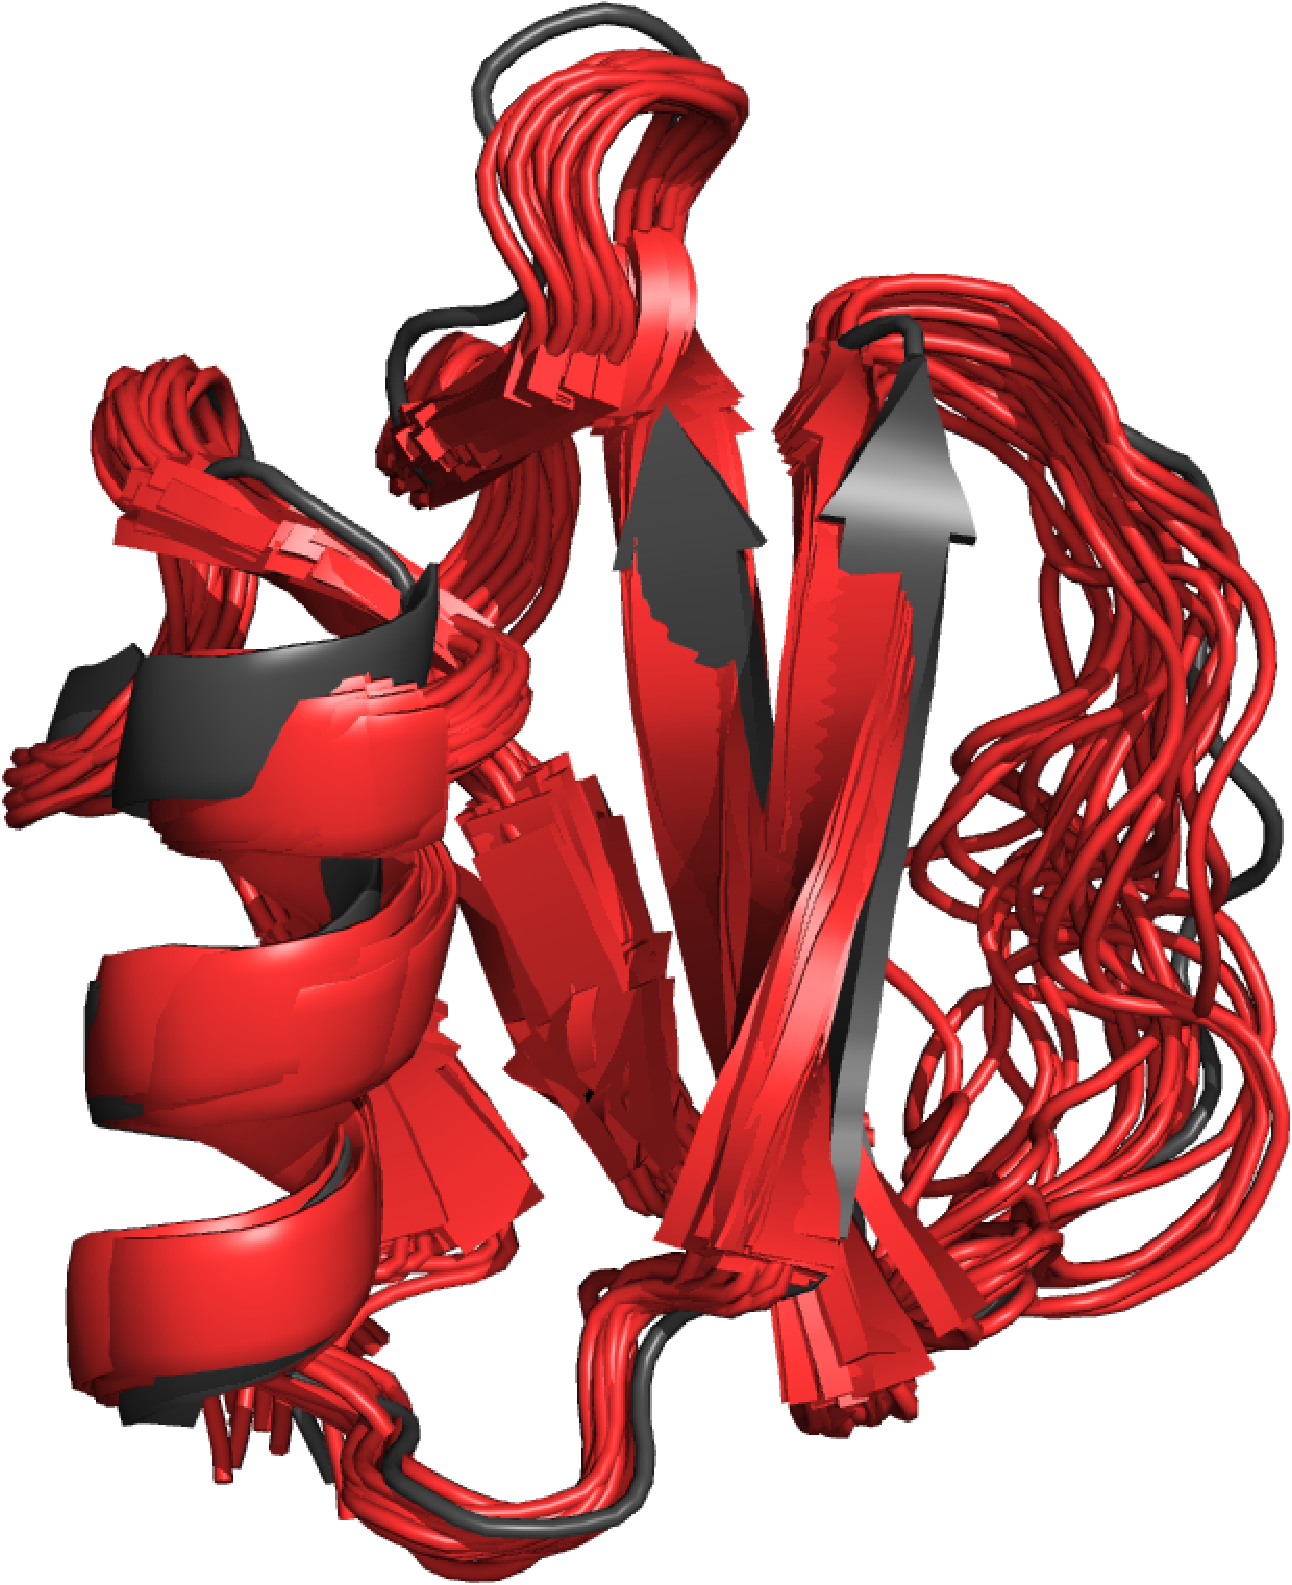
\includegraphics[width=0.3\textwidth]{figures/ci2_pymol/crystal_nmr_trim.pdf}}
    }
    \subfloat[Lowest RMSD structure (blue)]{
        {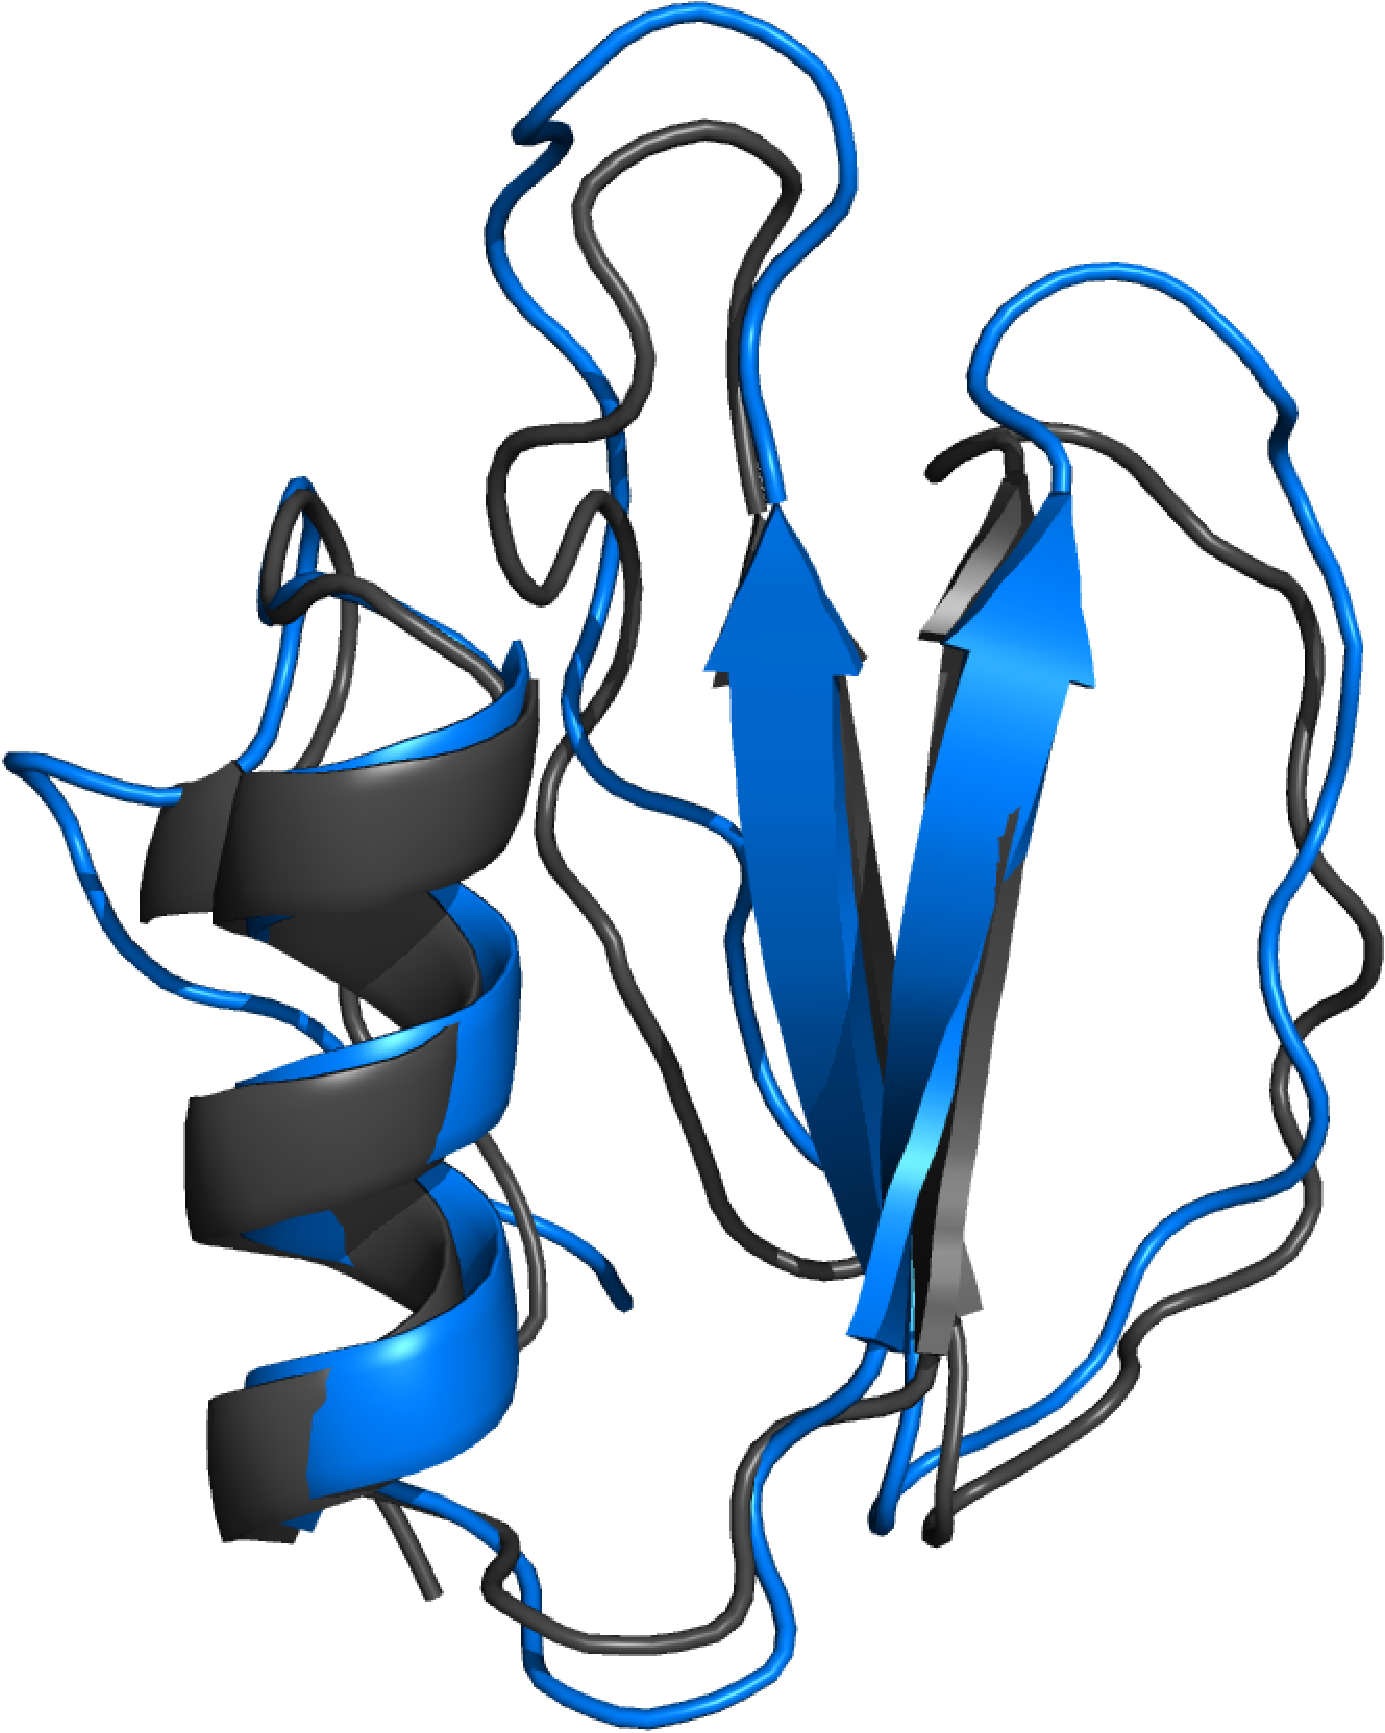
\includegraphics[width=0.3\textwidth]{figures/ci2_pymol/crystal_lowest_rmsd_trim.pdf}}
    }
    \subfloat[Lowest energy structure (green)]{
        {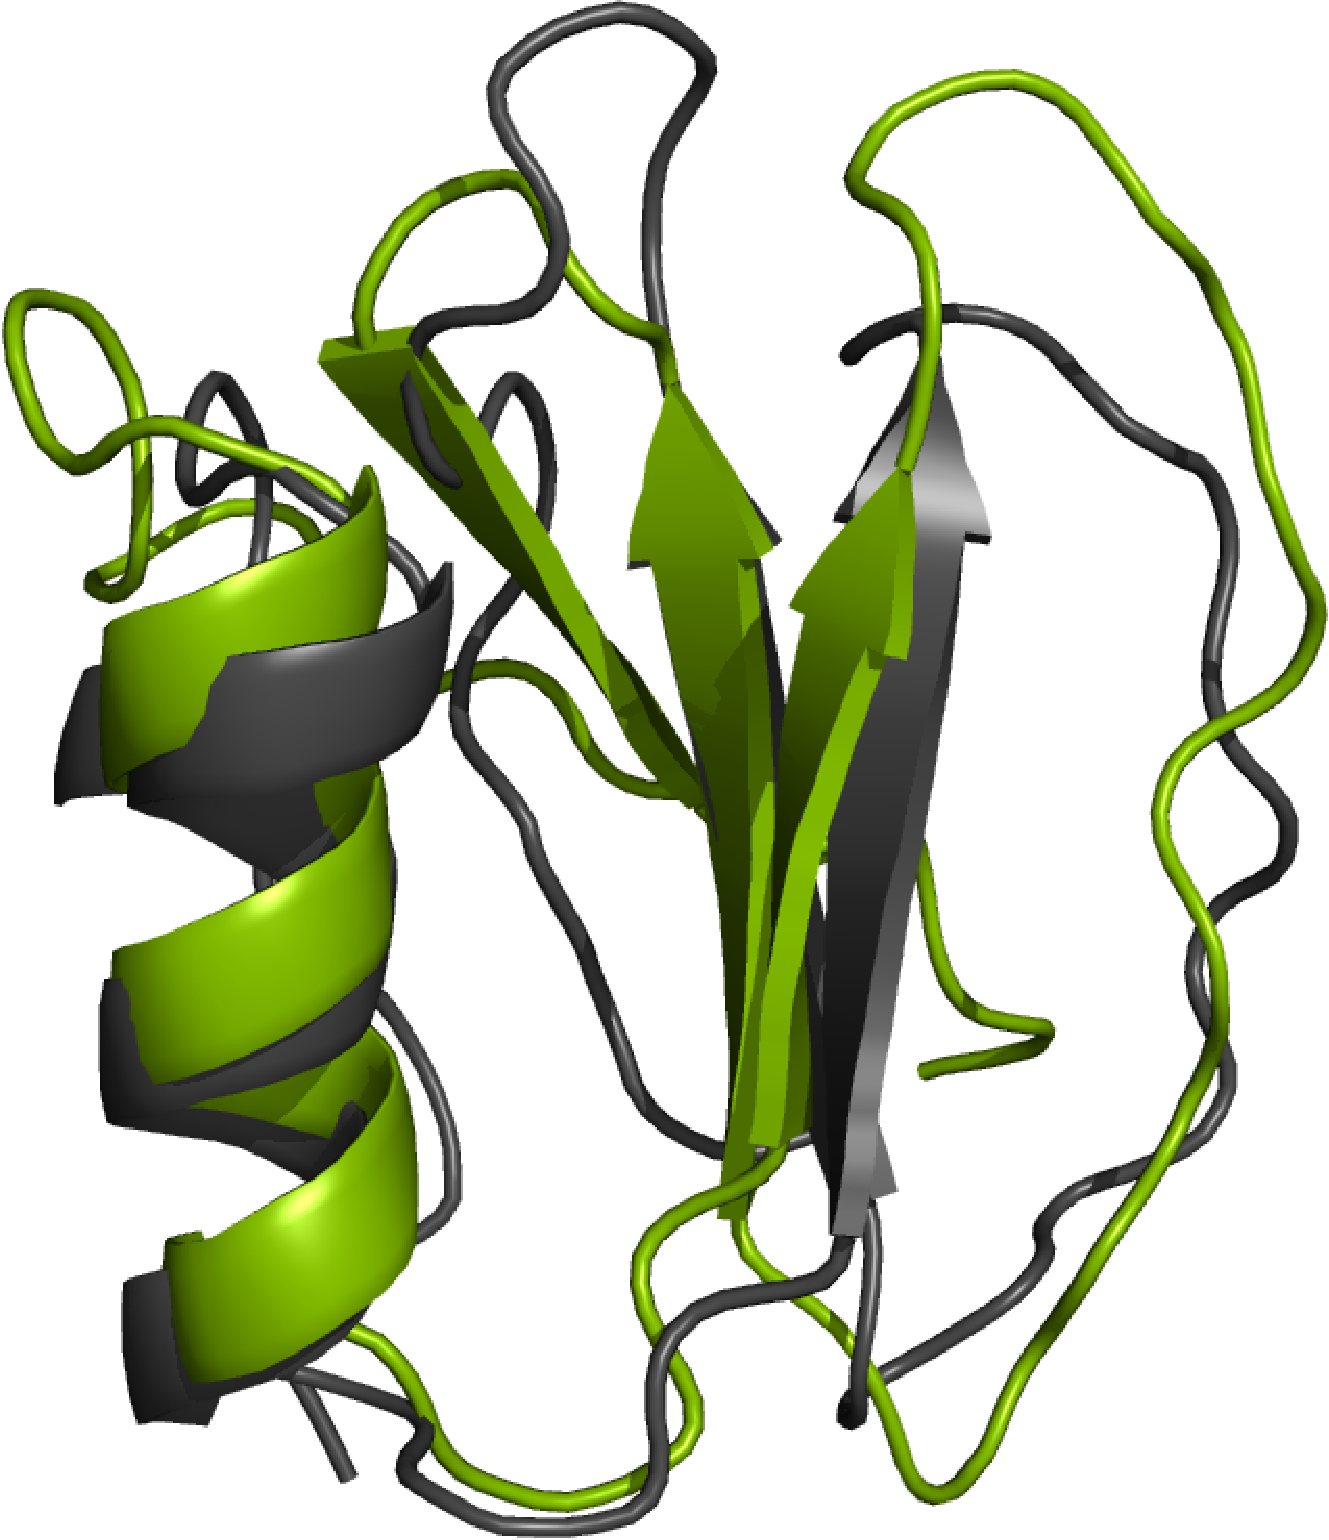
\includegraphics[width=0.3\textwidth]{figures/ci2_pymol/crystal_lowest_energy_trim.pdf}}
    }
    \caption{Structures compared to the X-ray structure 1YPA. All structures are aligned using the residues 12-32,43-52. (a) shows the 3CI2 structure NNR structure. Note the flexible domain which is excluded from the fit-range. (b) Shows the lowest RMSD structure (1.113 \AA RMSD). (c) shows the lowest energy sample (2.76 \AA RMSD). }
    \label{fig:ci2}%
\end{figure}

